\documentclass[11pt]{article}
\usepackage[utf8]{inputenc}
\usepackage[parfill]{parskip} % no indents
\usepackage{geometry}
 \geometry{
 a4paper,
 left=25mm,
 top=40mm,
 right=25mm,
 bottom=27mm
 }
\usepackage{natbib} % references
\usepackage{graphicx} % plots
\usepackage{scrextend} % indent authors
\usepackage{amsmath} % math typesetting
\usepackage{graphicx}
\usepackage{subcaption}
\usepackage{microtype}
% typeset in sans serif to match the prompt
\usepackage{lmodern}
\renewcommand{\familydefault}{\sfdefault}
% correct the section heading size
\usepackage{titlesec}
\titleformat*{\section}{\normalsize\bfseries}
%%%%%%%%%%%%%%%%%%%%%%%%%%%%%%%%%%%%%%%%%%%%%%%
\begin{document}
\raggedright % don't stretch to right edge

% =============================================
\vspace*{80pt}
{\LARGE \textbf{Global sensitivity analysis of model parameters in aeroelastic wind-turbine codes}}
\vspace*{28pt}

\begin{addmargin}[2.5cm]{0em}% 1em left, 2em right
\textbf{P. Kumar$^{\boldsymbol{\mathsf{1}}}$, B. Sanderse$^{\boldsymbol{\mathsf{1}}}$}

$^{\mathsf{1}}$ Centrum Wiskunde \& Informatica, Science Park 123, Amsterdam.

%$^{\mathsf{2}}$Address 2.
%\vspace{12pt}

Author contact email: b.sanderse@cwi.nl

Keywords: aero-elastic turbine model, BEM, sensitivity analysis, model uncertainty
\end{addmargin}

% =============================================
\section{Introduction}
Aeroelastic models such as the Blade Element Momentum (BEM) method \cite{HandBook} continue to play a critical role in the design, development and optimization of modern wind turbines. The accuracy of BEM predictions is affected by uncertainties and inaccuracies, for e.g., in the external conditions (wind parameters), in the turbine specifications (geometric parameters), and in the BEM equations itself (model parameters). For the purpose of design, uncertainty quantification and optimization, it is crucial to limit the number of parameters, typically by performing sensitivity studies. Most studies focused on the effect of uncertainties in the external conditions and geometry, see e.g. \cite{Echeverria2017,Robertson2018}. % removed reference Matthaus2017,Murcia2018 
\section{Objectives}
The long-term objective of this study is to develop calibrated BEM models that give users an indication of the uncertainty associated with the predictions (loads, power, etc.) originating not only from external conditions and geometry but also from the model formulation itself. For this purpose, we will calibrate the model parameters present in BEM models. Examples of such model parameters are the time constant in dynamic stall models, the wake correction factor, the tip loss model parameter, and the lift- and drag-polars \cite{Sayed2019}. To limit the number of model parameters involved in the calibration process, \textit{the objective of the current study is to perform a global sensitivity study of the outputs of the BEM model towards both geometric and model uncertainties}.

%In the past several sensitivity studies have been performed to understand the influence of input parameters on different turbine responses, e.g.\ \cite{moriarty2002effect, eggers2003wind, McKay2014, dykes2014sensitivity, Robertson2018}. Many studies have confirmed that wind parameters especially wind speed and wind speed standard deviation have the most influence on the aerodynamical performance of turbines. For example, in an upstream turbine, the wind speed is most sensitive to power production. Furthermore, wind speed in combination with wind speed standard deviation has a large influence on the power production of turbines operating in the wake of an upstream turbine. Among operational factors, the rotor RPM is the most sensitive to power production. [More on parameter sensitivities on structural loads]

% In particular, BEM models are employed to predict turbine response such as the structural loads and power outputs.

%`These tools use simplified methods such as BEM to find the unsteady aerodynamic loads and 1D structural models to determine the deformations. They are computationally cheap, but they are based on different corrections to account for the unsteadiness and the 3D effects.' \cite{Sayed2019}

%[Sensitivity on the polars as novel element]

%[Mention this study is a part of IEA Task29 project and WindTrue.

%In this work, we also study the effect of manufacturing tolerances on the turbine response. Usually, there is some discrepancy between the manufactured and nominally prescribed design of the turbine blade leading to suboptimal performance. For BEM models, the turbine shape is described as a series of airfoils along the span of the blade where each airfoil shape is computed using the three quantities: chord length, thickness, and twist. We perturb these three quantities to obtain a perturbed turbine blade and analyze with sections that have more influence on output quantities. 



% =============================================

% =============================================
\section{Methodology}
To compute parameter sensitivities we use a global sensitivity analysis (GSA) based on the Sobol expansion approach, which decomposes the total variance of the quantity of interest (model output) into contributions from individual parameters and their combinations, similar to \cite{Echeverria2017,Rinker2016}. We employ the uncertainty quantification toolbox \texttt{UQLab} \cite{uqlab}, which computes the Sobol indices from a sparse polynomial chaos expansion. \texttt{UQLab}'s modular structure allows for easy integration with available BEM codes. 

The geometric uncertainties currently considered are chord and twist distribution, whereas the model uncertainty enters via uncertainty in lift- and drag-polars. To express the chord, twist, lift and drag distributions along the turbine blade, an efficient parameterization is needed that gives flexible control over the prescribed uncertainty while limiting the number of required parameters. We have chosen to use Non-Uniform Rational Basis Splines (NURBS) for this purpose, similar to \cite{Echeverria2017}. 

% =============================================
\section{Results}
The aeroelastic code that we use is the \texttt{ECN Aero-Module} \cite{Boorsma2012} and the turbine is the 2MW NM80 turbine (blade radius of 38.8m) from the DANAERO project \cite{Troldborg2013}. The data for airfoil lift- and drag-polars are available at four locations along the blade at 11.87m, 17.82m, 28.97m and 35.53m. %The reference value of polars are obtained from wind-tunnel experiment with 3D corrections. 
The lift and drag variables at these sections are numbered Cl1 - Cl4 and Cd1 - Cd4 respectively. Uncertainty enters by multiplying the reference lift and drag curves by a random variable (see Fig. \ref{fig:samples}). The chord and twist are perturbed via a number of control points that define the NURBS representation; we use 5 chord (Ch1 - Ch5) and 6 twist (Tw1 - Tw6) control points and perturb each value randomly following a uniformly distribution. Examples of random samples for these input parameters are presented in Fig.~\ref{fig:samples}.

%Thus, by locally perturbing the chord and twist curves, we can identify locations along the blade that are sensitive to turbine response. For a given lift and drag curve, all control points are perturbed (globally) using the same random number. Here, we are interested in knowing at what locations the inaccuracies in polars may lead to the most variations in the turbine output.
In Fig.~\ref{fig:Sobol}, we show the total order Sobol indices as a measure of the sensitivity of the different geometric and model parameters on the power output. In this case, we observe the important result that the uncertainty in model parameters is at least as important as the uncertainty in geometric parameters. Furthermore, within the geometric parameters, the chord distribution shows a significantly higher sensitivity compared to the twist variables.

\begin{figure}[h!]
 \centering
 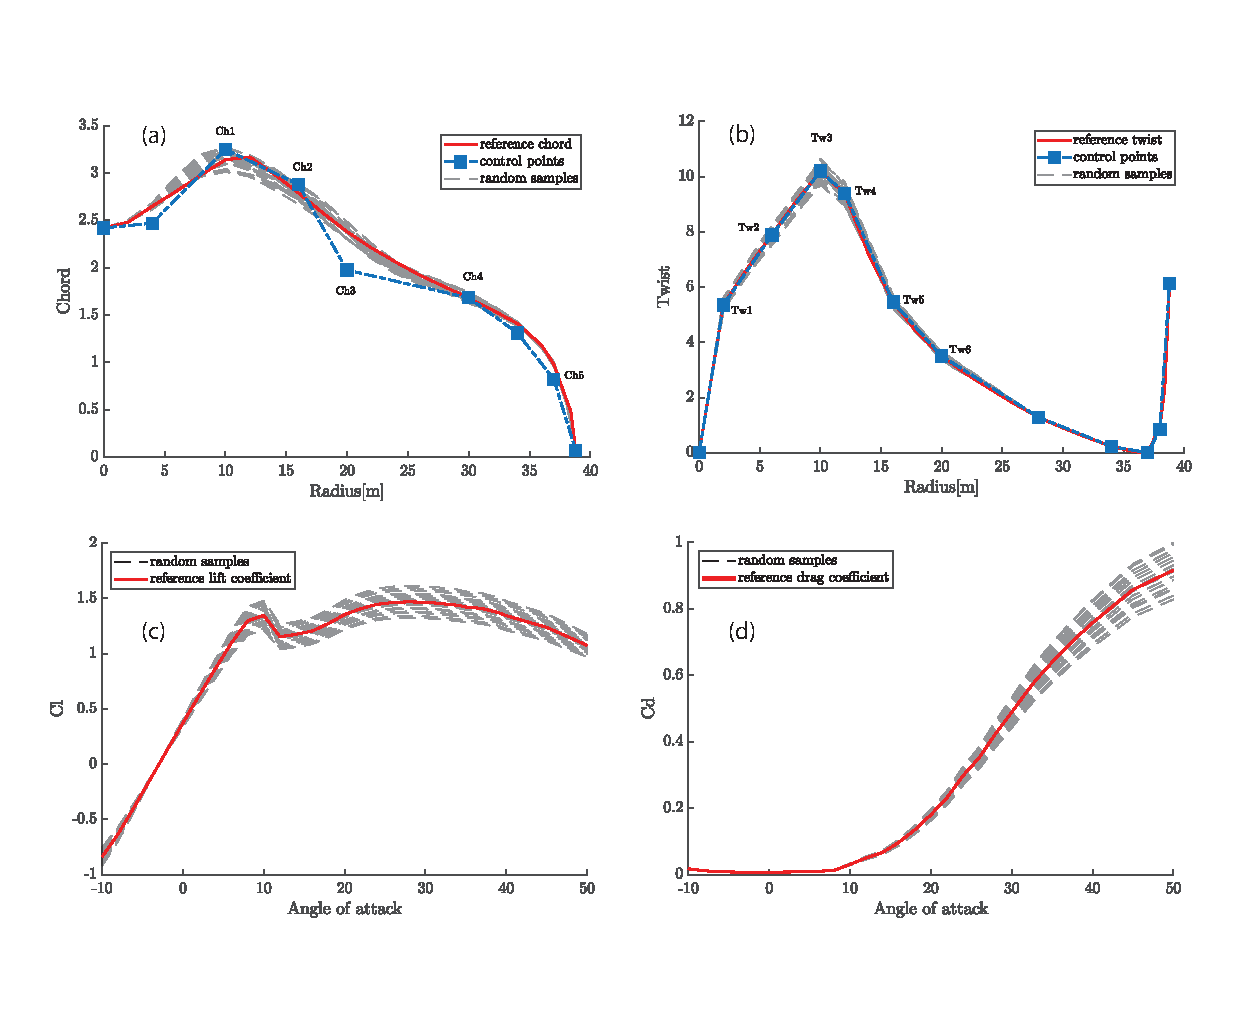
\includegraphics[trim={0 1.6cm 0 1.5cm},clip, scale=0.67]{figure1.pdf}
 \caption{Random realization of chord, twist, lift- (Cl2) and drag-polars (Cd2).}
 \label{fig:samples}
\end{figure}

\begin{figure}[h!]
 \centering
  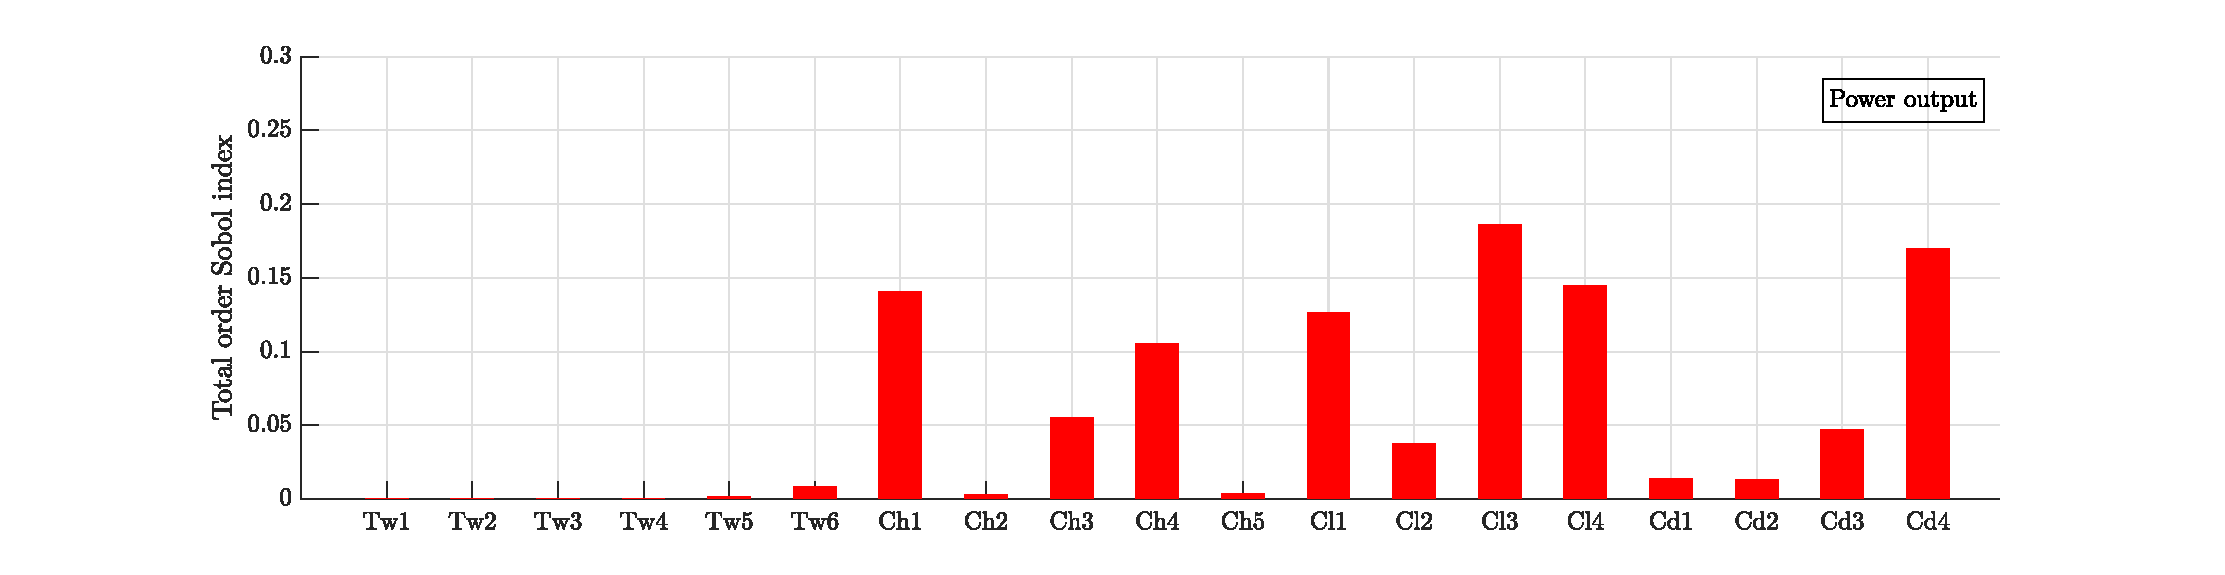
\includegraphics[width=\linewidth]{SA_Power_chord_twist_Cl_Cd.eps}
 \caption{Sensitivity of power output towards geometric and model parameters, expressed by Sobol indices.}
  \label{fig:Sobol}
\end{figure}
% =============================================
\section{Conclusions}
We have shown how Sobol indices computed using sparse adaptive polynomial expansion can be used for high-dimensional global sensitivity analysis of both geometric and model uncertainties. In the full paper, we will extend the sensitivity assessment to include more model uncertainties, such as parameters in dynamic stall and tip loss models. The identified sensitive model parameters will be utilized in future work to develop calibrated BEM models with built-in uncertainty estimates as part of the \textit{WindTrue} project, and is connected to IEA Task 29.

% =============================================
\bibliographystyle{abbrv}
\bibliography{../references,../Mendeley_refs}

\end{document}